\PassOptionsToPackage{unicode=true}{hyperref} % options for packages loaded elsewhere
\PassOptionsToPackage{hyphens}{url}
\PassOptionsToPackage{dvipsnames,svgnames*,x11names*}{xcolor}
%
\documentclass[]{article}
\usepackage{lmodern}
\usepackage{amssymb,amsmath}
\usepackage{ifxetex,ifluatex}
\usepackage{fixltx2e} % provides \textsubscript
\ifnum 0\ifxetex 1\fi\ifluatex 1\fi=0 % if pdftex
  \usepackage[T1]{fontenc}
  \usepackage[utf8]{inputenc}
  \usepackage{textcomp} % provides euro and other symbols
\else % if luatex or xelatex
  \usepackage{unicode-math}
  \defaultfontfeatures{Ligatures=TeX,Scale=MatchLowercase}
\fi
% use upquote if available, for straight quotes in verbatim environments
\IfFileExists{upquote.sty}{\usepackage{upquote}}{}
% use microtype if available
\IfFileExists{microtype.sty}{%
\usepackage[]{microtype}
\UseMicrotypeSet[protrusion]{basicmath} % disable protrusion for tt fonts
}{}
\IfFileExists{parskip.sty}{%
\usepackage{parskip}
}{% else
\setlength{\parindent}{0pt}
\setlength{\parskip}{6pt plus 2pt minus 1pt}
}
\usepackage{xcolor}
\usepackage{hyperref}
\hypersetup{
            colorlinks=true,
            linkcolor=Maroon,
            citecolor=Blue,
            urlcolor=cyan,
            breaklinks=true}
\urlstyle{same}  % don't use monospace font for urls
\usepackage[margin=1in]{geometry}
\usepackage{color}
\usepackage{fancyvrb}
\newcommand{\VerbBar}{|}
\newcommand{\VERB}{\Verb[commandchars=\\\{\}]}
\DefineVerbatimEnvironment{Highlighting}{Verbatim}{commandchars=\\\{\}}
% Add ',fontsize=\small' for more characters per line
\newenvironment{Shaded}{}{}
\newcommand{\AlertTok}[1]{\textcolor[rgb]{1.00,0.00,0.00}{\textbf{#1}}}
\newcommand{\AnnotationTok}[1]{\textcolor[rgb]{0.38,0.63,0.69}{\textbf{\textit{#1}}}}
\newcommand{\AttributeTok}[1]{\textcolor[rgb]{0.49,0.56,0.16}{#1}}
\newcommand{\BaseNTok}[1]{\textcolor[rgb]{0.25,0.63,0.44}{#1}}
\newcommand{\BuiltInTok}[1]{#1}
\newcommand{\CharTok}[1]{\textcolor[rgb]{0.25,0.44,0.63}{#1}}
\newcommand{\CommentTok}[1]{\textcolor[rgb]{0.38,0.63,0.69}{\textit{#1}}}
\newcommand{\CommentVarTok}[1]{\textcolor[rgb]{0.38,0.63,0.69}{\textbf{\textit{#1}}}}
\newcommand{\ConstantTok}[1]{\textcolor[rgb]{0.53,0.00,0.00}{#1}}
\newcommand{\ControlFlowTok}[1]{\textcolor[rgb]{0.00,0.44,0.13}{\textbf{#1}}}
\newcommand{\DataTypeTok}[1]{\textcolor[rgb]{0.56,0.13,0.00}{#1}}
\newcommand{\DecValTok}[1]{\textcolor[rgb]{0.25,0.63,0.44}{#1}}
\newcommand{\DocumentationTok}[1]{\textcolor[rgb]{0.73,0.13,0.13}{\textit{#1}}}
\newcommand{\ErrorTok}[1]{\textcolor[rgb]{1.00,0.00,0.00}{\textbf{#1}}}
\newcommand{\ExtensionTok}[1]{#1}
\newcommand{\FloatTok}[1]{\textcolor[rgb]{0.25,0.63,0.44}{#1}}
\newcommand{\FunctionTok}[1]{\textcolor[rgb]{0.02,0.16,0.49}{#1}}
\newcommand{\ImportTok}[1]{#1}
\newcommand{\InformationTok}[1]{\textcolor[rgb]{0.38,0.63,0.69}{\textbf{\textit{#1}}}}
\newcommand{\KeywordTok}[1]{\textcolor[rgb]{0.00,0.44,0.13}{\textbf{#1}}}
\newcommand{\NormalTok}[1]{#1}
\newcommand{\OperatorTok}[1]{\textcolor[rgb]{0.40,0.40,0.40}{#1}}
\newcommand{\OtherTok}[1]{\textcolor[rgb]{0.00,0.44,0.13}{#1}}
\newcommand{\PreprocessorTok}[1]{\textcolor[rgb]{0.74,0.48,0.00}{#1}}
\newcommand{\RegionMarkerTok}[1]{#1}
\newcommand{\SpecialCharTok}[1]{\textcolor[rgb]{0.25,0.44,0.63}{#1}}
\newcommand{\SpecialStringTok}[1]{\textcolor[rgb]{0.73,0.40,0.53}{#1}}
\newcommand{\StringTok}[1]{\textcolor[rgb]{0.25,0.44,0.63}{#1}}
\newcommand{\VariableTok}[1]{\textcolor[rgb]{0.10,0.09,0.49}{#1}}
\newcommand{\VerbatimStringTok}[1]{\textcolor[rgb]{0.25,0.44,0.63}{#1}}
\newcommand{\WarningTok}[1]{\textcolor[rgb]{0.38,0.63,0.69}{\textbf{\textit{#1}}}}
\usepackage{longtable,booktabs}
% Fix footnotes in tables (requires footnote package)
\IfFileExists{footnote.sty}{\usepackage{footnote}\makesavenoteenv{longtable}}{}
\usepackage{graphicx,grffile}
\makeatletter
\def\maxwidth{\ifdim\Gin@nat@width>\linewidth\linewidth\else\Gin@nat@width\fi}
\def\maxheight{\ifdim\Gin@nat@height>\textheight\textheight\else\Gin@nat@height\fi}
\makeatother
% Scale images if necessary, so that they will not overflow the page
% margins by default, and it is still possible to overwrite the defaults
% using explicit options in \includegraphics[width, height, ...]{}
\setkeys{Gin}{width=\maxwidth,height=\maxheight,keepaspectratio}
\setlength{\emergencystretch}{3em}  % prevent overfull lines
\providecommand{\tightlist}{%
  \setlength{\itemsep}{0pt}\setlength{\parskip}{0pt}}
\setcounter{secnumdepth}{0}
% Redefines (sub)paragraphs to behave more like sections
\ifx\paragraph\undefined\else
\let\oldparagraph\paragraph
\renewcommand{\paragraph}[1]{\oldparagraph{#1}\mbox{}}
\fi
\ifx\subparagraph\undefined\else
\let\oldsubparagraph\subparagraph
\renewcommand{\subparagraph}[1]{\oldsubparagraph{#1}\mbox{}}
\fi

% set default figure placement to htbp
\makeatletter
\def\fps@figure{htbp}
\makeatother


\date{}

\begin{document}

\hypertarget{two---introduction-to-reinforcement-learning}{%
\section{Two - Introduction to Reinforcement
Learning}\label{two---introduction-to-reinforcement-learning}}

Context, the Markov Decision Process, four central challenges in
reinforcement learning.

\begin{center}\rule{0.5\linewidth}{\linethickness}\end{center}

\hypertarget{what-is-reinforcement-learning}{%
\subsection{What is reinforcement
learning}\label{what-is-reinforcement-learning}}

\begin{quote}
Of all the forms of machine learning, reinforcement learning is the
closest to the kind of learning that humans and other animals do, and
many of the core algorithms of reinforcement learning were originally
inspired by biological learning systems - Sutton \& Barto -
Reinforcement Learning: An Introduction
\end{quote}

The reinforcement learning approach is one that is familiar to any human
being. It is learning through action.

\begin{itemize}
\tightlist
\item
  to learn chess in a supervised manner, we would learn moves from
  textbooks of the games of grandmasters.
\item
  to learn chess in a reinforcement learning manner, we would learn
  chess by playing ourselves.
\end{itemize}

Reinforcement learning is fundamentally about \textbf{decision making}.
An agent learns to act in sequential decision making problem.

The goal in reinforcement learning is to develop agents that can learn
to take actions that maximize a scalar reward signal.

\begin{quote}
Goal at DeepMind is to try to use reinforcement learning to solve some
of the bigger visions of AI \ldots{} it is the paradigm of artificial
intelligence \ldots{} RL is the paradigm that describes how to learn
optimal decisions in any environment -
\href{https://www.youtube.com/watch?v=M5a6HasTHs4}{David Silver}
\end{quote}

Agents \textbf{generate data through action}. They also create
\textbf{targets for supervised learning}. There are multiple moving
parts in an agent, which makes reinforcement learning non-IID and
non-stationary.

\hypertarget{biological-inspiration}{%
\subsection{Biological inspiration}\label{biological-inspiration}}

\begin{quote}
Neurobiological evidence that reward signals during perceptual learning
may influence the characteristics of representations within the primate
visual cortex - Mnih et. al (2015) Human-level control through deep
reinforcement learning
\end{quote}

\hypertarget{habit-formation}{%
\subsubsection{Habit formation}\label{habit-formation}}

The mechanism by which habits are formed is essentially the
reinforcement learning mechanism

Cue -\textgreater{} Routine -\textgreater{} Reward

State -\textgreater{} Action -\textgreater{} Reward

Variable rewards

\begin{itemize}
\tightlist
\item
  dopamine surges when brain is expecting a reward
\item
  variability multiplies the effect
\item
  focused state where judgment and reason are suppressed
\end{itemize}

\hypertarget{schultz-1990-experiments}{%
\subsubsection{Schultz 1990
experiments}\label{schultz-1990-experiments}}

\href{https://www.youtube.com/watch?v=ul6B2oFPNDM}{A History of
Reinforcement Learning - Prof.~A.G. Barto} -
\href{https://github.com/ADGEfficiency/dsr-rl/blob/master/literature/classic_rl/1997_Schultz_neural_substrate_reward.pdf}{Schultz
(1997) - A Neural Substrate of Prediction and Reward}

\textbf{Dopamine} - connection between TD error and dopamine in the
brain. Dopamine signal can be modelled as a TD error. Phasic activity of
dopamine is trigged by a reward. With continued trials, the dopamine
signal moves back towards the time of the prediction (which is the same
that the TD error does - a backup).
(https://www.youtube.com/watch?v=ul6B2oFPNDM)

The phasic activity of mesencephalic dopamine neurons signals the error
between and old and new estimate of expected future reward

\begin{figure}
\centering
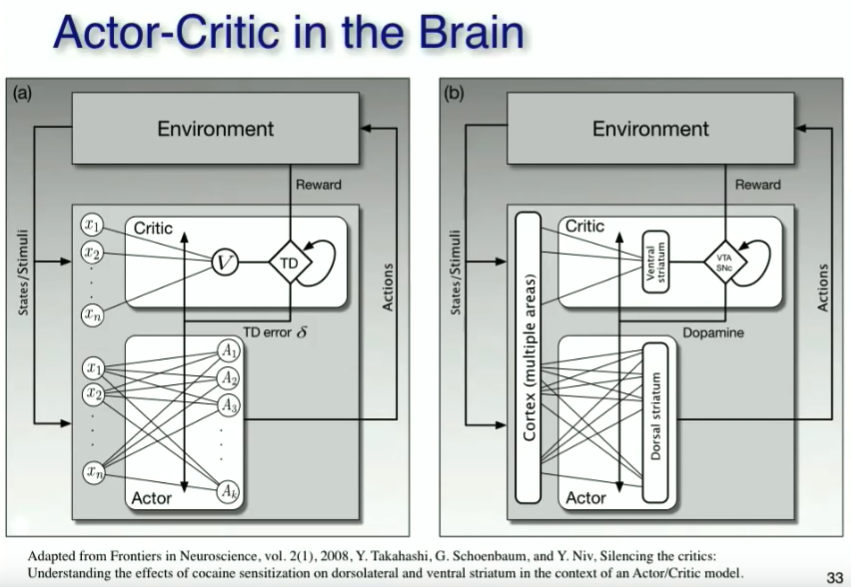
\includegraphics[width=\textwidth,height=0.3\textheight]{./tex2pdf.-4c1708fb449e9e84/44dd1b489d5e060cd9fcd09b66bacb48267e0ca5.png}
\caption{Theory around how the actor-critic model might work in the
brain}
\end{figure}

\hypertarget{applications}{%
\subsection{Applications}\label{applications}}

David Silver gives the following

\begin{itemize}
\tightlist
\item
  control physical systems
\item
  interact with users - customer retention, personalization
\item
  solve logistical problems - scheduling, bandwidth allocation, power
  optimization
\item
  play games
\item
  learn sequential algorithms - attention, memory, conditional
  computation, activations
\end{itemize}

All of these problems involve \textbf{decision making}.

\newpage

\hypertarget{related-methods}{%
\subsection{Related methods}\label{related-methods}}

\begin{figure}
\centering
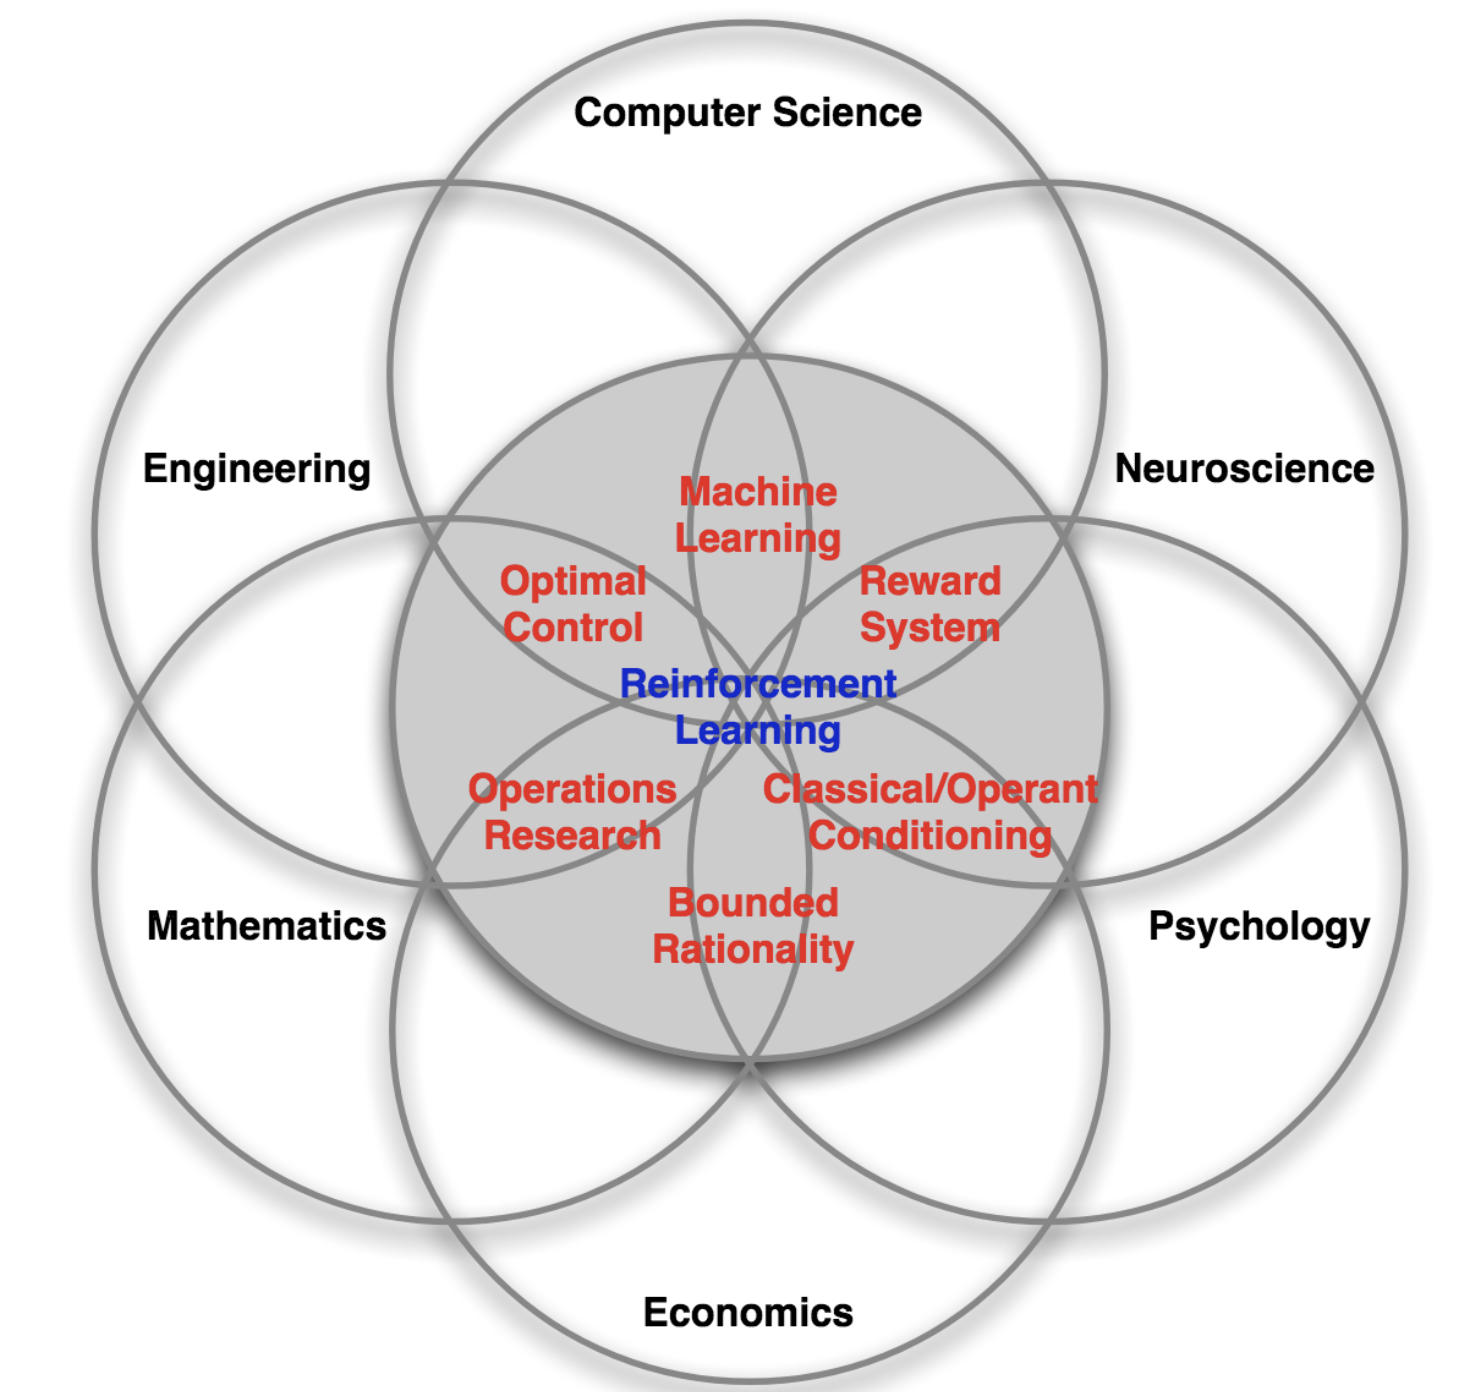
\includegraphics[width=\textwidth,height=0.35\textheight]{./tex2pdf.-4c1708fb449e9e84/4e5835c194f814b7abab51f3cbf790fcc60291b9.png}
\caption{Faces of RL - David Silver Lecture 1}
\end{figure}

A \textbf{domain specific} algorithm for your problem - if you have one,
use it! Reinforcement learning is about generalization - but this
generalization comes at a cost (that domain specific problems don't
have).

\textbf{Evolutionary methods} -
\href{https://en.wikipedia.org/wiki/Evolutionary_algorithm}{wikipedia}

\begin{itemize}
\tightlist
\item
  use biological inspired mechanisms such as reproduction, mutation and
  selection
\item
  better able to deal with sparse error signals
\item
  easily parallelizable
\item
  tend to perform better that RL if state variable is hidden
\item
  CMA-ES works well for solution spaces up to a few thousand parameters
\end{itemize}

\textbf{Cross entropy method}
\href{https://en.wikipedia.org/wiki/Cross-entropy_method}{wikipedia}

\begin{itemize}
\tightlist
\item
  often recommended as an alternative
\item
  generate a random sampling of data (i.e.~an episode)
\item
  update parameters of the model to produce a better sample in the next
  iteration
\item
  this involves minimizing the KL-divergence
\item
  also see \textbf{Covariance Matrix Adaptation (CMA)}
\end{itemize}

\textbf{Linear programming}
\href{https://en.wikipedia.org/wiki/Linear_programming}{wikipedia}

\begin{itemize}
\tightlist
\item
  constrained optimization
\item
  environment model must be linear
\end{itemize}

\textbf{Optimal control}
\href{https://en.wikipedia.org/wiki/Optimal_control}{wikipedia} -
\href{https://www.youtube.com/watch?v=oulLR06lj_E}{Data-Driven control
lecture}

\begin{itemize}
\tightlist
\item
  primarily concerned with control of linear systems
\item
  commonly used in electrical engineering
\end{itemize}

\newpage

\hypertarget{context-within-machine-learning}{%
\subsection{Context within machine
learning}\label{context-within-machine-learning}}

\begin{figure}
\centering
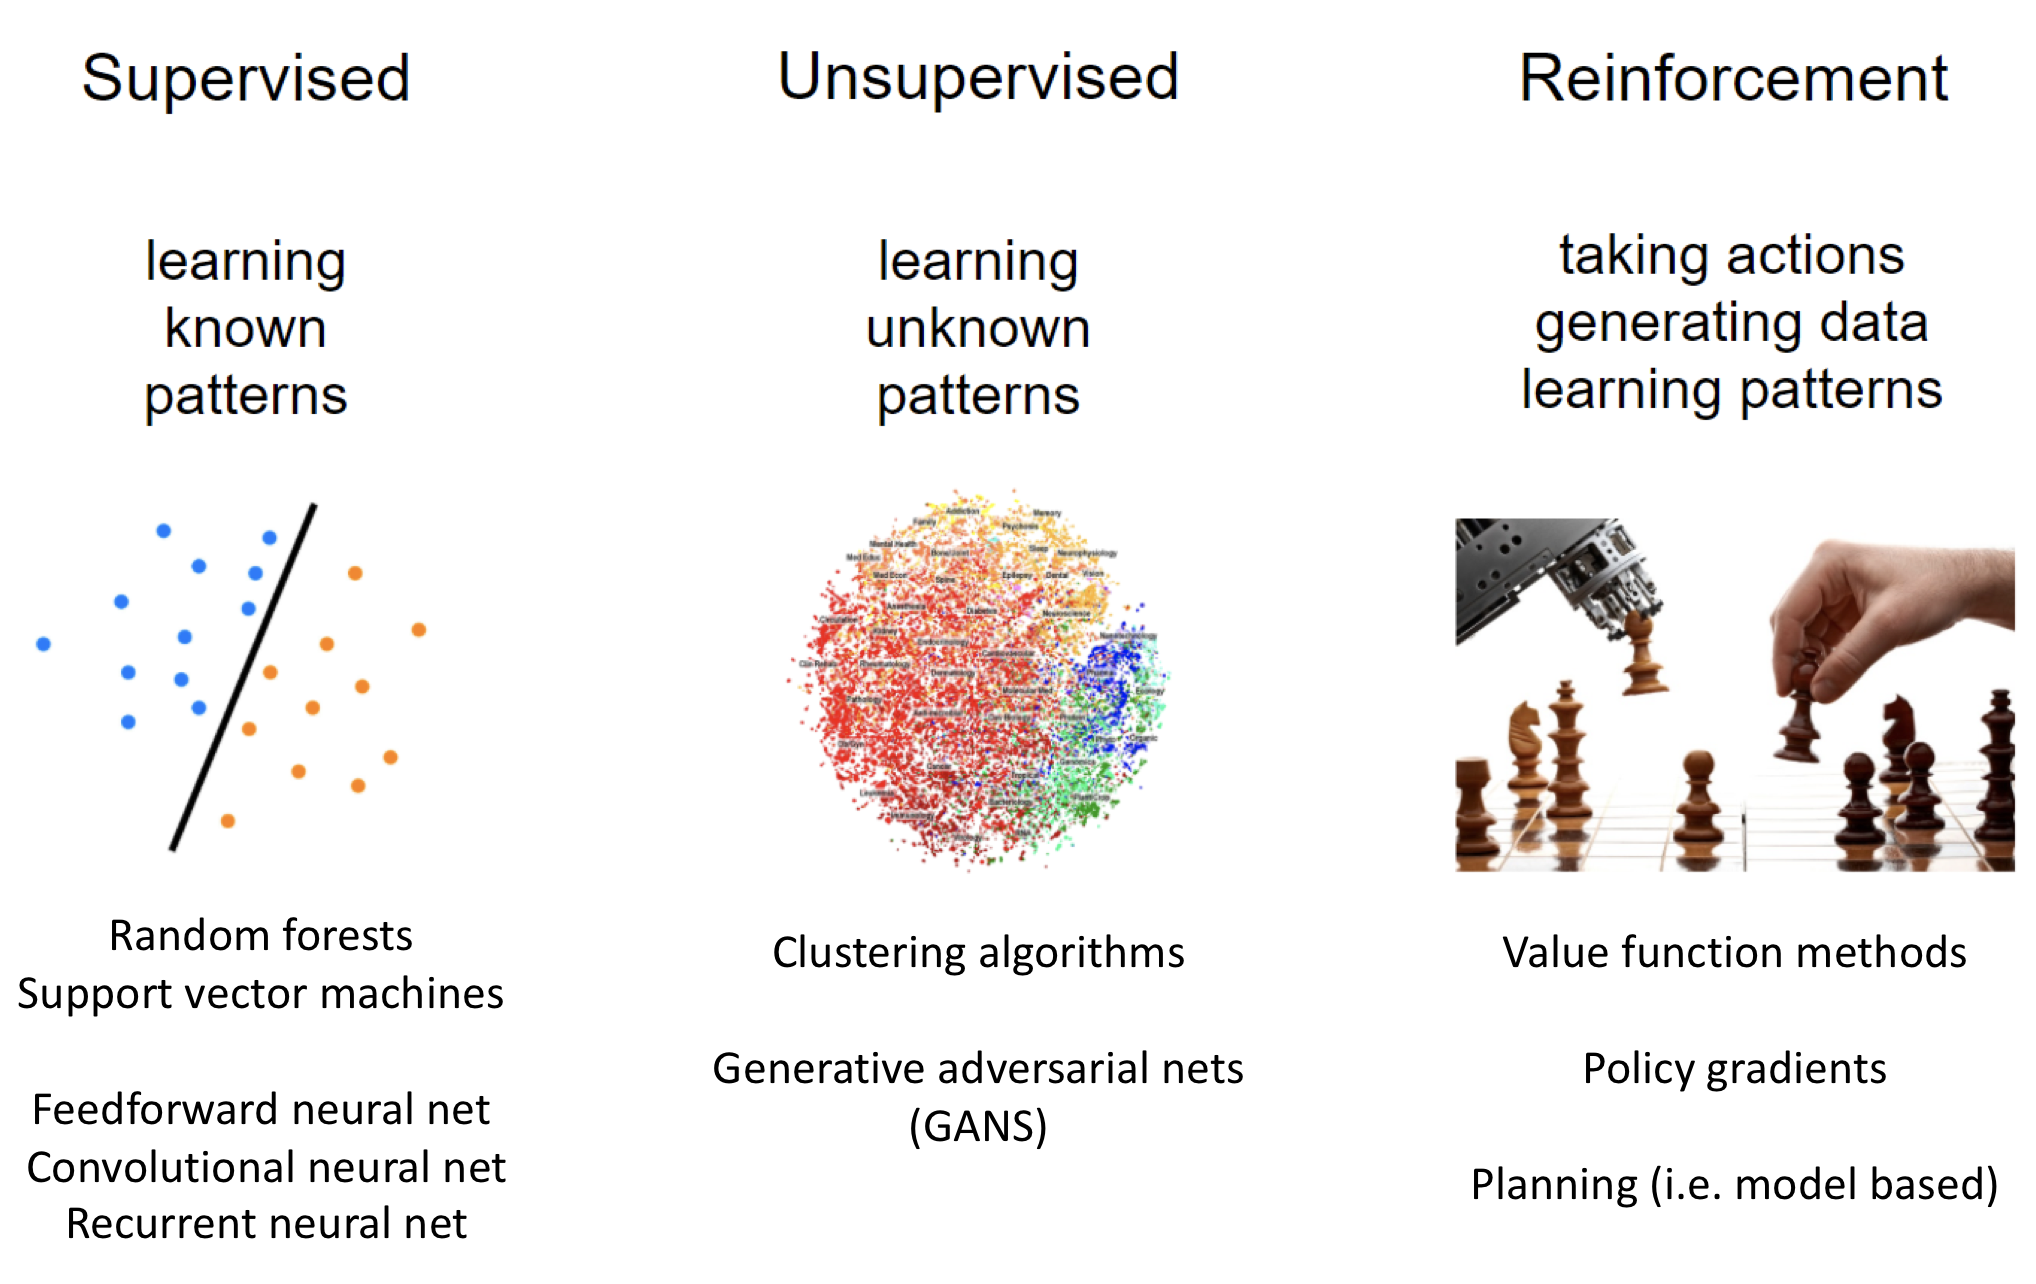
\includegraphics[width=\textwidth,height=0.3\textheight]{./tex2pdf.-4c1708fb449e9e84/6e3b6e89fcfbd67b1f2060ede8d3c3a9f88c321d.png}
\caption{Three areas of machine learning. The difference is the feedback
signal available to the learner.}
\end{figure}

\hypertarget{supervised-learning}{%
\subsubsection{Supervised learning}\label{supervised-learning}}

Dataset and labels.

Feedback is the target (one per sample).

\begin{itemize}
\tightlist
\item
  are given a dataset with labels
\item
  we are constrained by this dataset
\item
  test on unseen data
\end{itemize}

\begin{longtable}[]{@{}ll@{}}
\toprule
features & target\tabularnewline
\midrule
\endhead
\((2.0, 1.5)\) & \(25\)\tabularnewline
\((1.2, 0.3)\) & \(7.2\)\tabularnewline
\bottomrule
\end{longtable}

\hypertarget{unsupervised-learning}{%
\subsubsection{Unsupervised learning}\label{unsupervised-learning}}

Dataset, no labels.

Feedback from data structures, adversarial training.

\begin{longtable}[]{@{}l@{}}
\toprule
features\tabularnewline
\midrule
\endhead
\((2.0, 1.5)\)\tabularnewline
\((1.2, 0.3)\)\tabularnewline
\bottomrule
\end{longtable}

\hypertarget{reinforcement-learning}{%
\subsubsection{Reinforcement learning}\label{reinforcement-learning}}

No dataset, no labels.

Feedback from state transitions and a scalar reward signal.

\begin{itemize}
\tightlist
\item
  are given no dataset and no labels
\item
  we can generate more data by acting
\item
  test using the same environment
\end{itemize}

Reinforcement learning has more to do that supervised learning. In
reinforcement learning we need to \textbf{generate our own data}. The
data we generate is experience tuples \((s,a,r,s')\), which are sampled
from the environment by taking actions. How we generate that data
(i.e.~what actions we take) is up to the agent.

Once we store a list of these experience tuples in our agents memory, we
then need to learn. In supervised learning all our samples have targets
(i.e.~the class of that sample). The reinforcement learning dataset is
just a list of tuples!

This is the second task that agents need to do - \textbf{label their
experience}. Once the experience is labelled, supervised learning
techniques (such as stochastic gradient descent) can be used to fit a
function that predicts the target. Reinforcement learning uses
supervised learning as a tool to learn functions.

\[[experience, experience, ..., experience]\]
\[[(s_0, a_0, r_1, s_1), (s_1, a_1, r_2, s_2), ..., (s_n, a_n, r_n, s_n)] \]

Success in modern reinforcement learning (2013 onwards) is in part due
to making use of advances in supervised learning (deep neural networks)
to better approximate functions the agent chooses to learn.

\hypertarget{reinforcement-learning-is-not}{%
\subsubsection{Reinforcement learning is
not}\label{reinforcement-learning-is-not}}

NOT an alternative method to use instead of a random forest, neural
network etc. ``I'll try to solve this problem using a convolutional nn
or RL'' - \textbf{this is nonsensical}.

Neural networks (supervised techniques in general) are a tool that
reinforcement learners can use to learn or approximate functions

\begin{itemize}
\tightlist
\item
  classifier learns the function of image -\textgreater{} cat
\item
  regressor learns the function of market\_data -\textgreater{}
  stock\_price
\end{itemize}

In reinforcement learning a common function we want to learn is a policy
- a function of state -\textgreater{} action. Another is a value
function, which maps state -\textgreater{} return.

\hypertarget{deep-reinforcement-learning}{%
\subsubsection{Deep reinforcement
learning}\label{deep-reinforcement-learning}}

\textbf{Deep learning} = neural networks with multiple layers

\textbf{Deep reinforcement learning} = using multiple layer networks to
approximate policies or value functions

\begin{itemize}
\tightlist
\item
  feedforward
\item
  convolutional
\item
  recurrent
\end{itemize}

\newpage

\hypertarget{model-free-reinforcement-learning}{%
\subsubsection{Model free reinforcement
learning}\label{model-free-reinforcement-learning}}

\begin{figure}
\centering
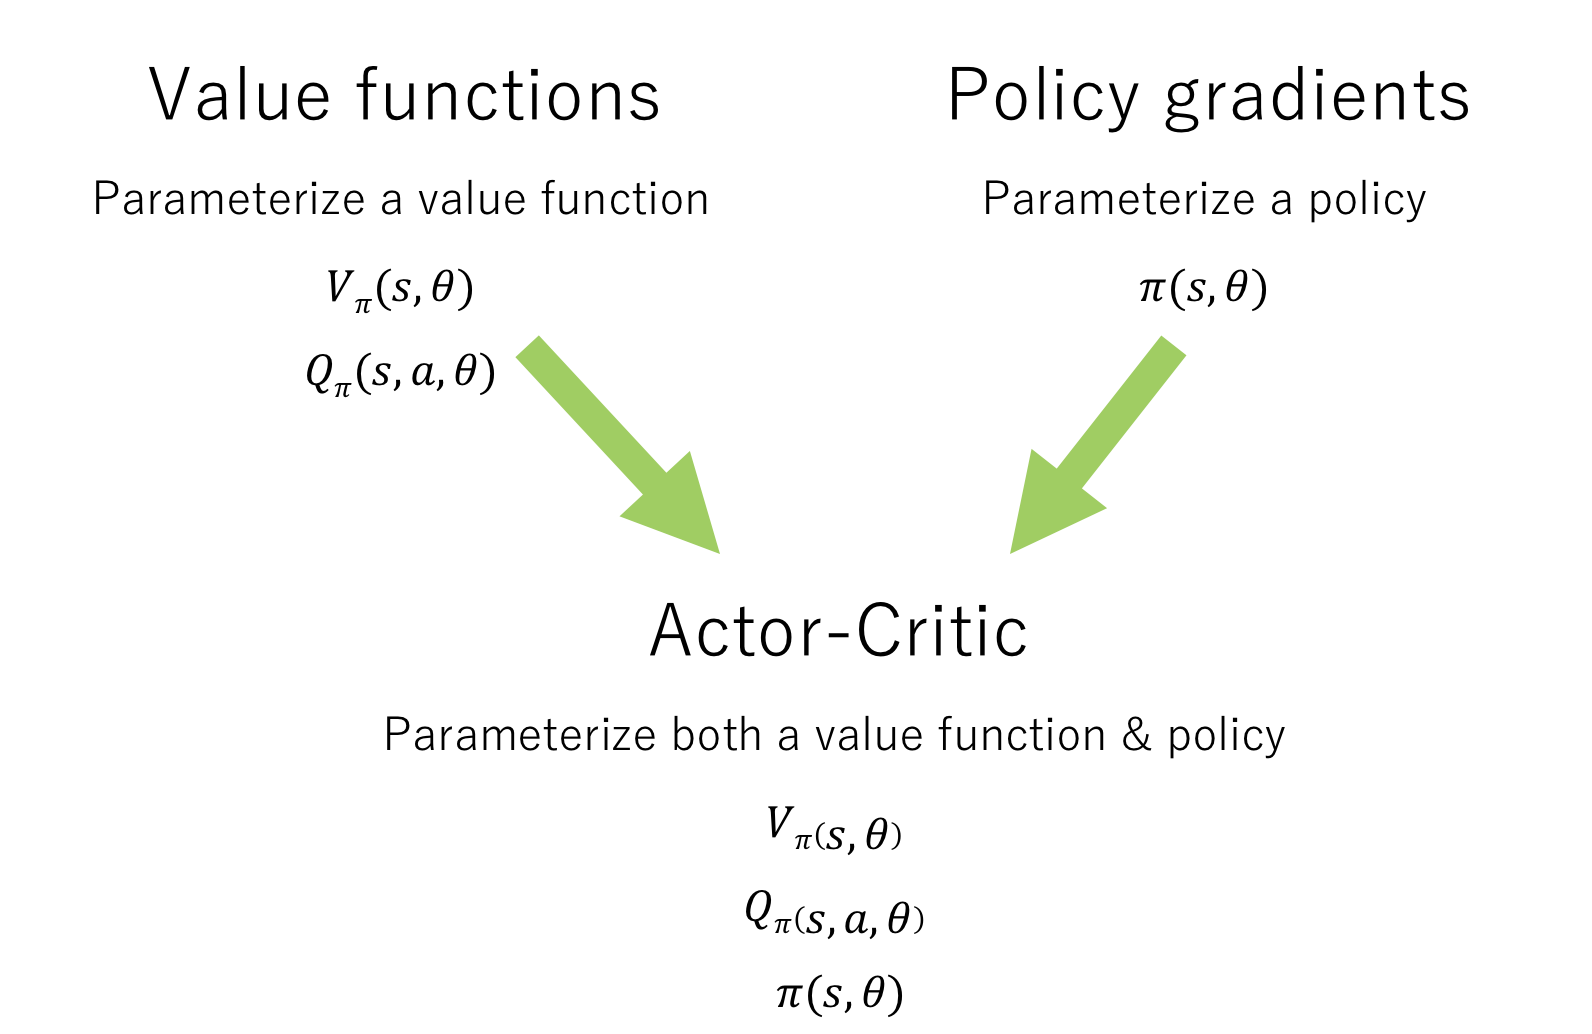
\includegraphics[width=\textwidth,height=0.3\textheight]{./tex2pdf.-4c1708fb449e9e84/7045eaef9110e46e3c6e0f51f24effa39b42af6b.png}
\caption{Model based reinforcement learning is outside the scope of this
course.}
\end{figure}

\newpage

\hypertarget{markov-decision-processes}{%
\subsection{Markov Decision Processes}\label{markov-decision-processes}}

The mathematical framework for reinforcement learning.

\hypertarget{markov-property}{%
\subsubsection{Markov property}\label{markov-property}}

Future is conditional only on the present

Can make prediction or decisions using only the current state

Any additional information about the history of the process will not
improve our decision

\[ P(s_{t+1} | s_{t}, a_{t}) = P(s_{t+1}|s_t, a_t...s_0, a_0)\]

Can be a requirement to guarantee convergence (often also require tables
or linear function approximators).

\begin{figure}
\centering
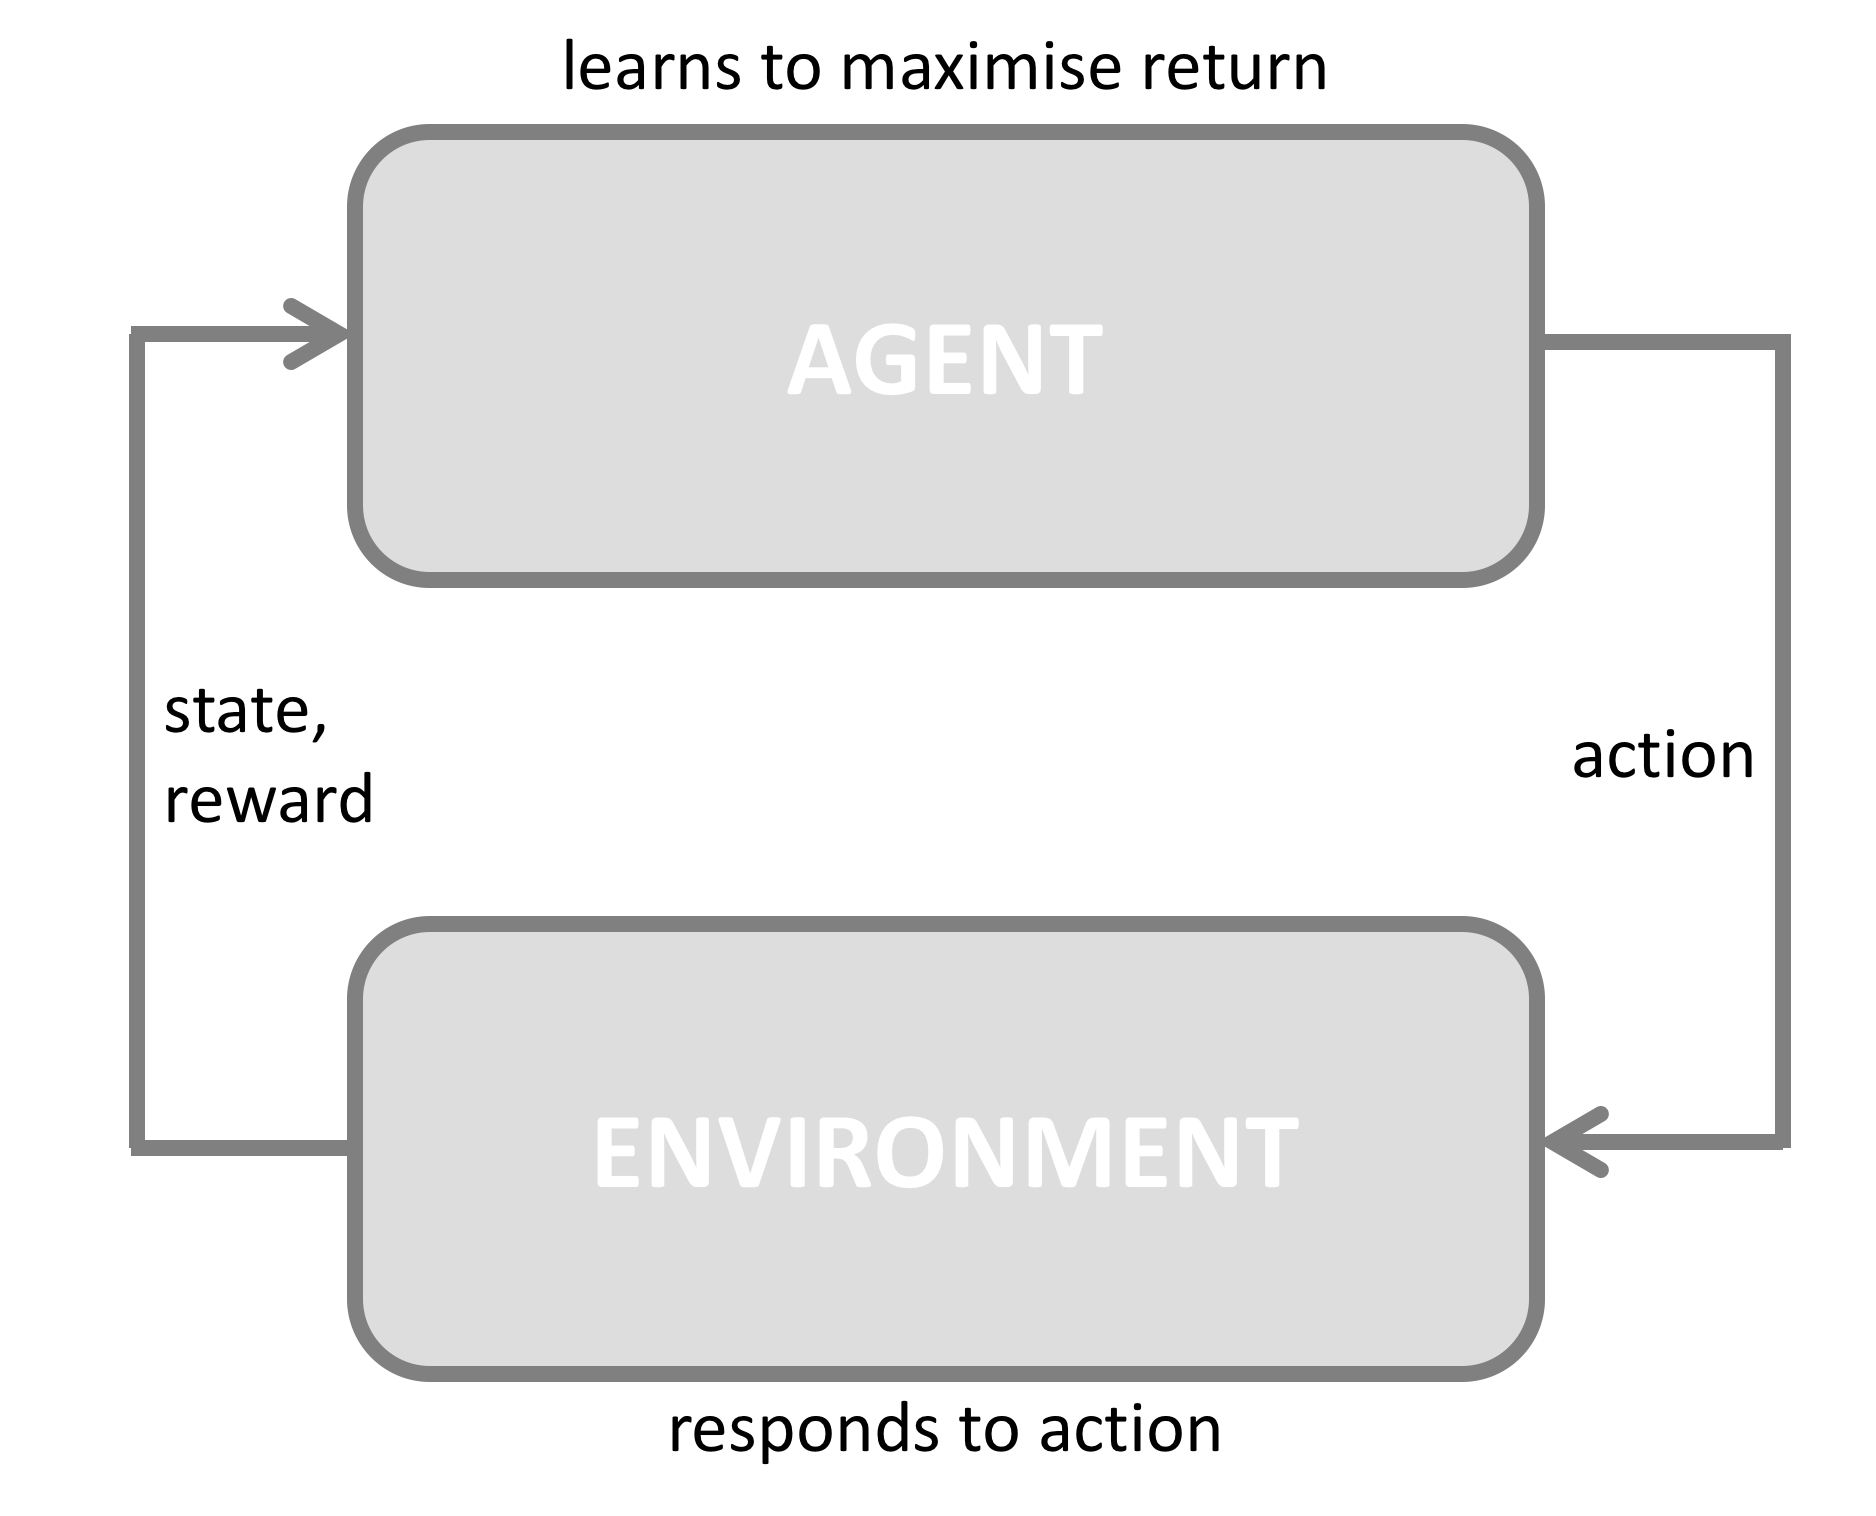
\includegraphics[width=\textwidth,height=0.2\textheight]{./tex2pdf.-4c1708fb449e9e84/5c97f063036ae7d1380a3d9d280f30b5101b81b9.png}
\caption{The basic Markov Decision Process framework for reinforcement
learning}
\end{figure}

\begin{figure}
\centering
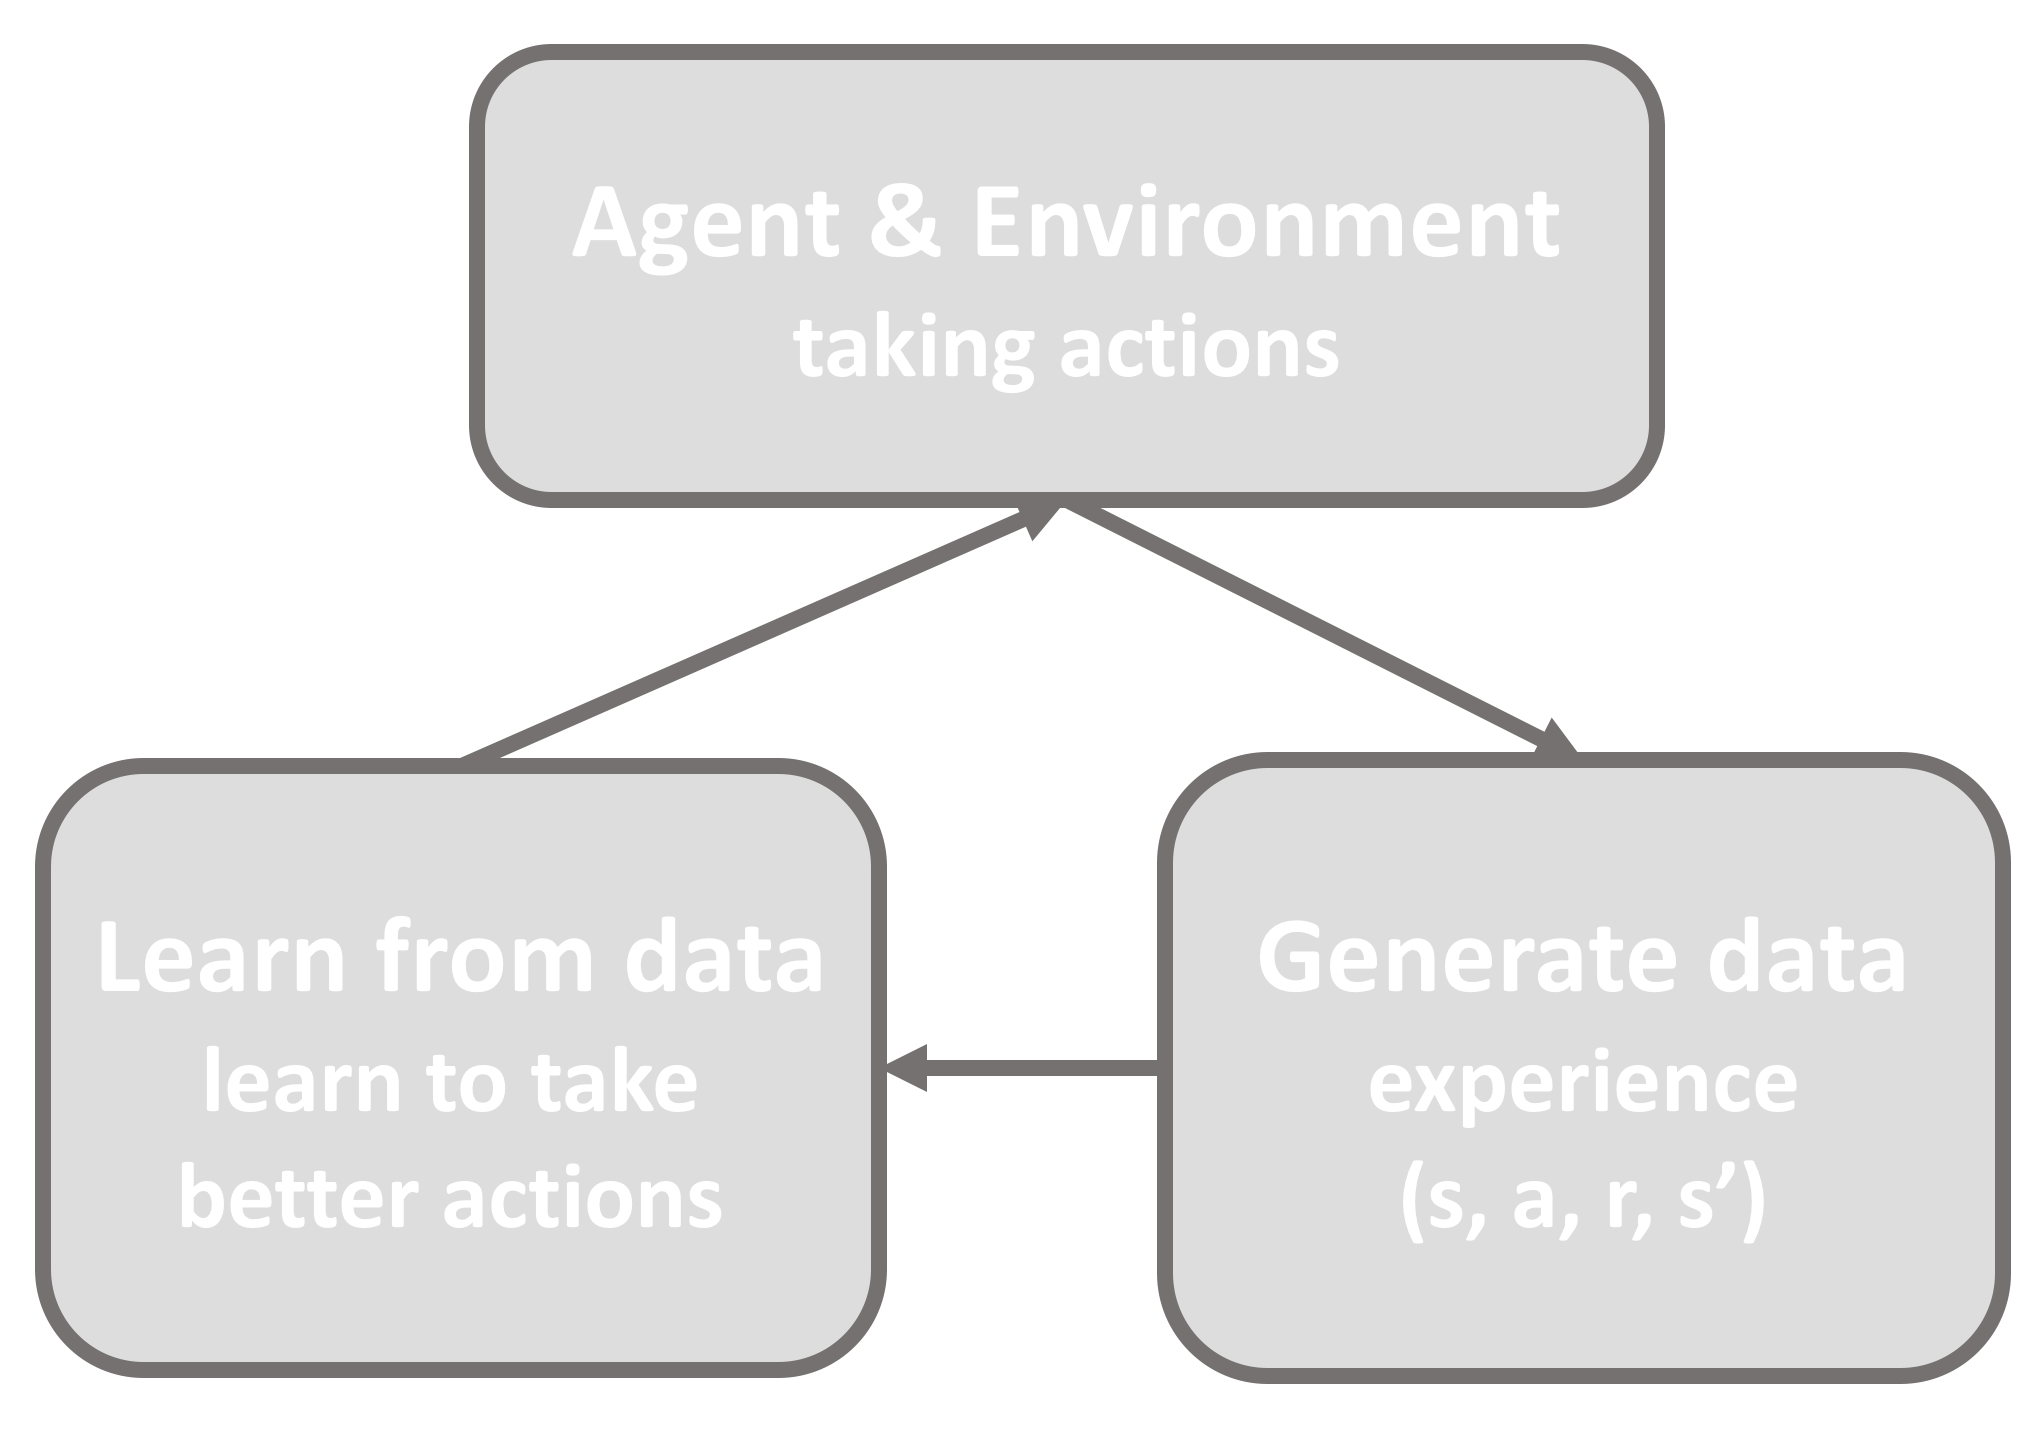
\includegraphics[width=\textwidth,height=0.2\textheight]{./tex2pdf.-4c1708fb449e9e84/78093fdd7ea165ed93d07e7605ed0289ecc8deb0.png}
\caption{The MDP generates data which an agent uses to learn}
\end{figure}

\newpage

\hypertarget{formal-definition-of-a-mdp}{%
\subsubsection{Formal definition of a
MDP}\label{formal-definition-of-a-mdp}}

An MDP can be defined as a tuple

\[(\mathcal{S}, \mathcal{A}, \mathcal{R}, P, R, d_0, \gamma)\]

Set of states \(\mathcal{S}\)

Set of actions \(\mathcal{A}\)

Set of rewards \(\mathcal{R}\)

State transition function \(P(s'|s,a)\)

Reward transition function \(R(r|s,a,s')\)

Distribution over initial states \(d_0\)

Discount factor \(\gamma\)

\hypertarget{object-oriented-definition-of-a-mdp}{%
\subsection{Object oriented definition of a
MDP}\label{object-oriented-definition-of-a-mdp}}

Two objects - the agent and environment

Three signals - state, action \& reward

\begin{Shaded}
\begin{Highlighting}[]
\KeywordTok{class}\NormalTok{ Agent}

\KeywordTok{class}\NormalTok{ Environment}

\NormalTok{state }\OperatorTok{=}\NormalTok{ env.reset()}

\NormalTok{action }\OperatorTok{=}\NormalTok{ agent.act(state)}

\NormalTok{reward, next_state }\OperatorTok{=}\NormalTok{ env.step(action)}
\end{Highlighting}
\end{Shaded}

\hypertarget{environment}{%
\subsubsection{Environment}\label{environment}}

Real or virtual

\begin{itemize}
\tightlist
\item
  modern RL uses virtual environments to generate lots of experience
\end{itemize}

Each environment has a state space and an action space

\begin{itemize}
\tightlist
\item
  these spaces can be discrete or continuous
\end{itemize}

Environments can be

\begin{itemize}
\tightlist
\item
  episodic (finite length, can be variable or fixed length)
\item
  non-episodic (infinite length)
\end{itemize}

The MDP framework unites both in the same way by using the idea of a
final absorbing state at the end of episodes

Discretiziation

\begin{itemize}
\tightlist
\item
  some agents require discrete spaces (i.e.~Q-Learning requires a
  discrete action space)
\item
  too coarse -\textgreater{} non-smooth control output
\item
  too fine -\textgreater{} curse of dimensionality \& computational
  expense
\item
  requires some prior knowledge
\item
  lose the shape of the space
\end{itemize}

Losing the shape of the space = agent sees all actions as discrete
options, and has no way to understand the relationship between each one
(this is true for the DQN style neural network, with one output node per
action).

\hypertarget{state}{%
\subsubsection{State}\label{state}}

Infomation for the agent to \textbf{choose next action} and to
\textbf{learn from}

State is a flexible concept - it's a n-d array

\begin{Shaded}
\begin{Highlighting}[]
\NormalTok{state }\OperatorTok{=}\NormalTok{ np.array([temperature, pressure])}

\NormalTok{state }\OperatorTok{=}\NormalTok{ np.array(pixels).reshape(height, width)}
\end{Highlighting}
\end{Shaded}

Make sure all the info you need to learn \& make good decisions is in
the state!

\hypertarget{observation}{%
\subsubsection{Observation}\label{observation}}

Many problems your agent won't be able to see everything that would help
it learn - i.e.~non-Markov

This then becomes a POMDP - partially observed MDP

\begin{Shaded}
\begin{Highlighting}[]
\NormalTok{state }\OperatorTok{=}\NormalTok{ np.array([temperature, pressure])}

\NormalTok{observation }\OperatorTok{=}\NormalTok{ np.array([temperature }\OperatorTok{+}\NormalTok{ noise])}
\end{Highlighting}
\end{Shaded}

Observation can be made more Markov by - concatenating state
trajectories together - using function approximation with a memory
element (LSTMs)

\hypertarget{agent}{%
\subsubsection{Agent}\label{agent}}

Our agent is the \textbf{learner and decision maker}

It's goal is to maximize total discounted reward

An agent always has a policy

\hypertarget{reward}{%
\subsubsection{Reward}\label{reward}}

The reward is a scalar signal sent at each step (it can be zero). The
reward for an action can often be \textbf{delayed} - making assigning
credit to the correct action difficult.

The reward signal can also be \textbf{sparse} - the most extreme cases
being environments where all rewards are zero except the terminal state
(such as Go or Chess).

A well defined reward signal is a limit for applying reinforcement
learning. Autonomous driving is a good example - the reward function for
driving has to be designed to balance safety, speed etc.

\begin{quote}
The Reward Engineering Principle = As reinforcement learning based AI
systems become more general and more autonomous, the design of reward
mechanisms that elicit desired behaviours becomes both more important
and more difficult -
\href{http://www.danieldewey.net/reward-engineering-principle.pdf}{Reinforcement
Learning and the Reward Engineering Principle}
\end{quote}

Maximising expected return is also making an assumption about the nature
of our goals

\emph{Goals can be described by the maximization of expected cumulative
reward} - do you agree with this? Think about

\begin{itemize}
\tightlist
\item
  happiness
\item
  status
\item
  reputation
\end{itemize}

Think about the role of emotion in human decision making. Is there a
place for this in reinforcement learning

\hypertarget{policy-pis}{%
\subsubsection{\texorpdfstring{Policy
\(\pi(s)\)}{Policy \textbackslash{}pi(s)}}\label{policy-pis}}

\[\pi(s)\] \[\pi(s,a|\theta)\] \[\pi_\theta(s|a)\]

A policy is

\begin{itemize}
\tightlist
\item
  rules to select actions (in this state, go left etc)
\item
  a function that maps state -\textgreater{} action
\item
  a probability distribution over actions
\end{itemize}

Some example policies are

\begin{itemize}
\tightlist
\item
  always act randomly
\item
  always pick a specific action
\item
  the optimal policy - the policy that maximizes future reward
\end{itemize}

Policies can be parameterized directly (policy gradient methods) or
generated from a value function (value function methods). They can also
be either deterministic or stochastic.

\hypertarget{on-versus-off-policy-learning}{%
\subsubsection{On versus off policy
learning}\label{on-versus-off-policy-learning}}

On policy - learn about the policy we are using to make decisions

Off policy - evaluate or improve one policy while using another to make
decisions

Control can be on or off policy - use general policy iteration to
improve a policy using an on-policy approximation. On to off-policyness
is a scale (agents vary in degrees).

\begin{quote}
Maybe the less we need to learn from deep learning is large capacity
learners with large and diverse datasets - Sergey Levine
\end{quote}

Why would we want to learn off-policy?

\begin{itemize}
\tightlist
\item
  we can learn about policies that we don't have
\item
  learn the optimal policy from data generated by a random policy
\item
  we can reuse data
\item
  on-policy algorithms have to throw away experience after the policy is
  improved
\end{itemize}

Learning from diverse datasets = requires off-policy learning.

\begin{figure}
\centering
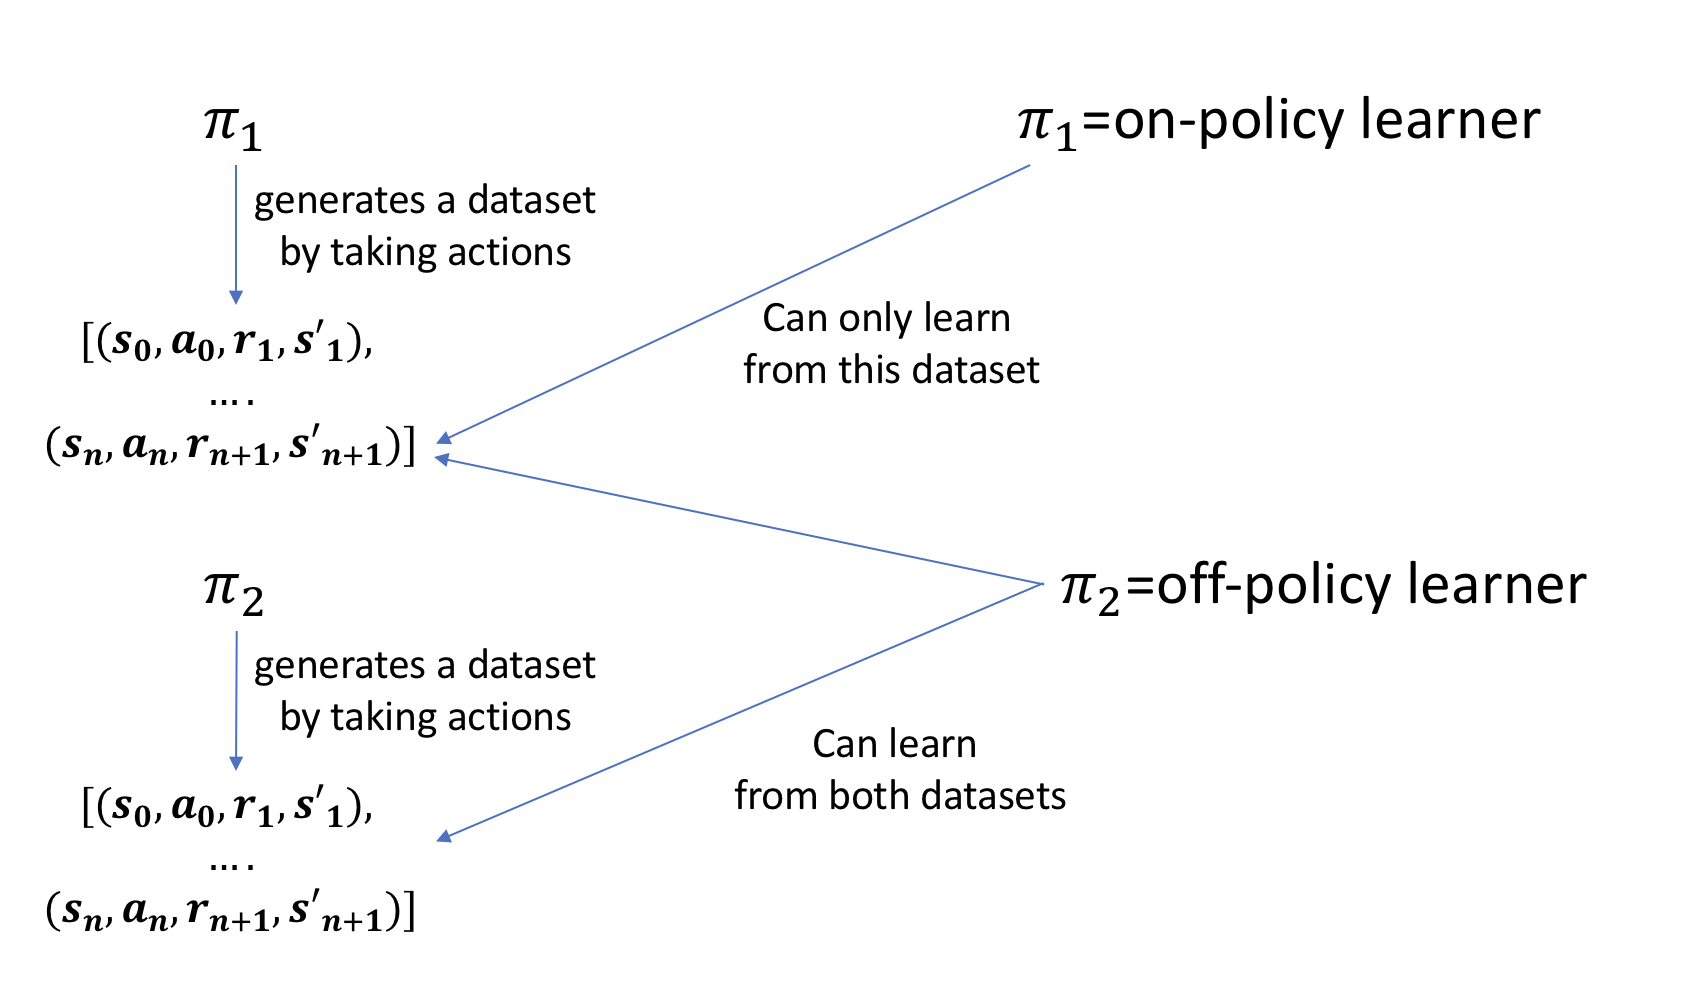
\includegraphics[width=\textwidth,height=0.4\textheight]{./tex2pdf.-4c1708fb449e9e84/bad6552c70d63ef31aafc1f9a8d6f3e06a3157f1.png}
\caption{Two policies that generate datasets of experience by acting in
the environment. One policy can only learn from it's own experience -
the second policy can learn from both datasets}
\end{figure}

Remember that as soon as the weights of any neural networks used by the
agent changes, the policy changes. On-policy agents must throw away
experience after they have improved the policy.

An off-policy agent can reuse experience multiple times - is able to use
experience generated by a poor quality policy being followed for
exploration early on in an agent's life.

\hypertarget{environment-model}{%
\subsection{Environment model}\label{environment-model}}

Environment models predict the response (i.e.~next state and reward) of
an environment for a given state and action.

\[ P(s',r | s, a) \]

Our agent can learn an environment model - predicts environment response
to actions - predicts \(s', r\) from \(s, a\)

\begin{Shaded}
\begin{Highlighting}[]
\KeywordTok{def}\NormalTok{ model(state, action):}
    \CommentTok{# do stuff}
    \ControlFlowTok{return}\NormalTok{ next_state, reward}
\end{Highlighting}
\end{Shaded}

Sample vs.~distributional model

\begin{itemize}
\tightlist
\item
  sample can be easy to build (i.e.~two random number generators for
  rolling dice)
\item
  distributional requires understanding the probability distribution
  over all possible next states and rewards
\end{itemize}

Model can be used to simulate trajectories for \textbf{planning}.
Planning is really important in our own thinking, and is very powerful
if you can get it to work.

A good environment model is very valuable - it allows planning. Planning
is the simulation of rollouts - the agent can use the results of these
rollouts to decide what action to take or to improve learning.

A key challenge in model based reinforcement learning is to learn the
model. If a good model can be learnt then it's likely to be very
valuable. Dynamic programming (which is introduced in Section 3) uses an
environment model to perfectly solve environments.

\begin{figure}
\centering
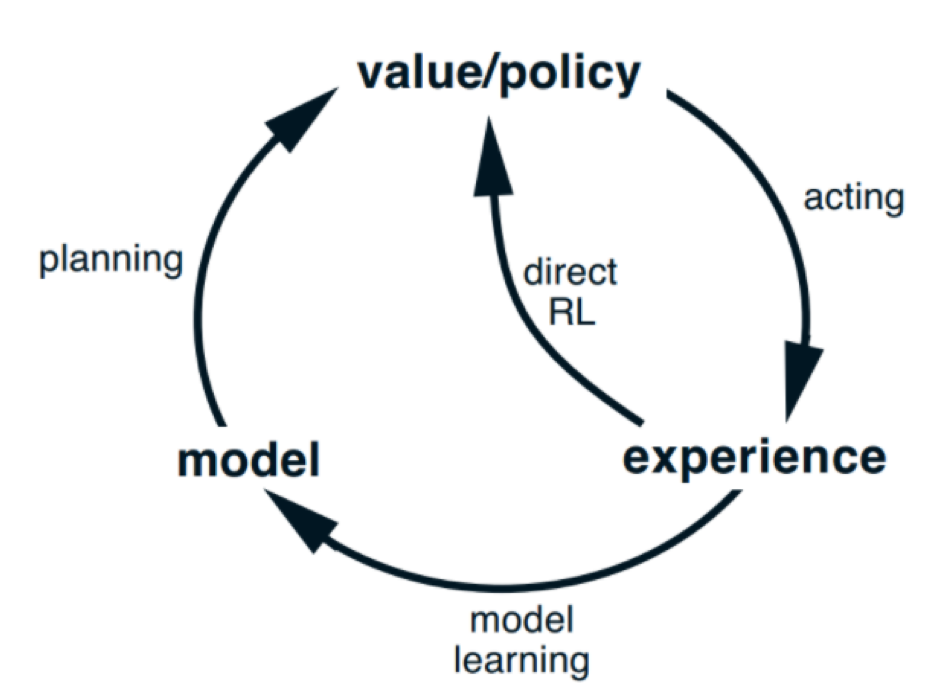
\includegraphics[width=\textwidth,height=0.3\textheight]{./tex2pdf.-4c1708fb449e9e84/7ef01ac31f42757acbd4ebba9ecb26d67dd6ae46.png}
\caption{Relationships amoung learning, planning and action - Sutton \&
Barto - Reinforcement Learning: An Introduction}
\end{figure}

\newpage

\begin{figure}
\centering
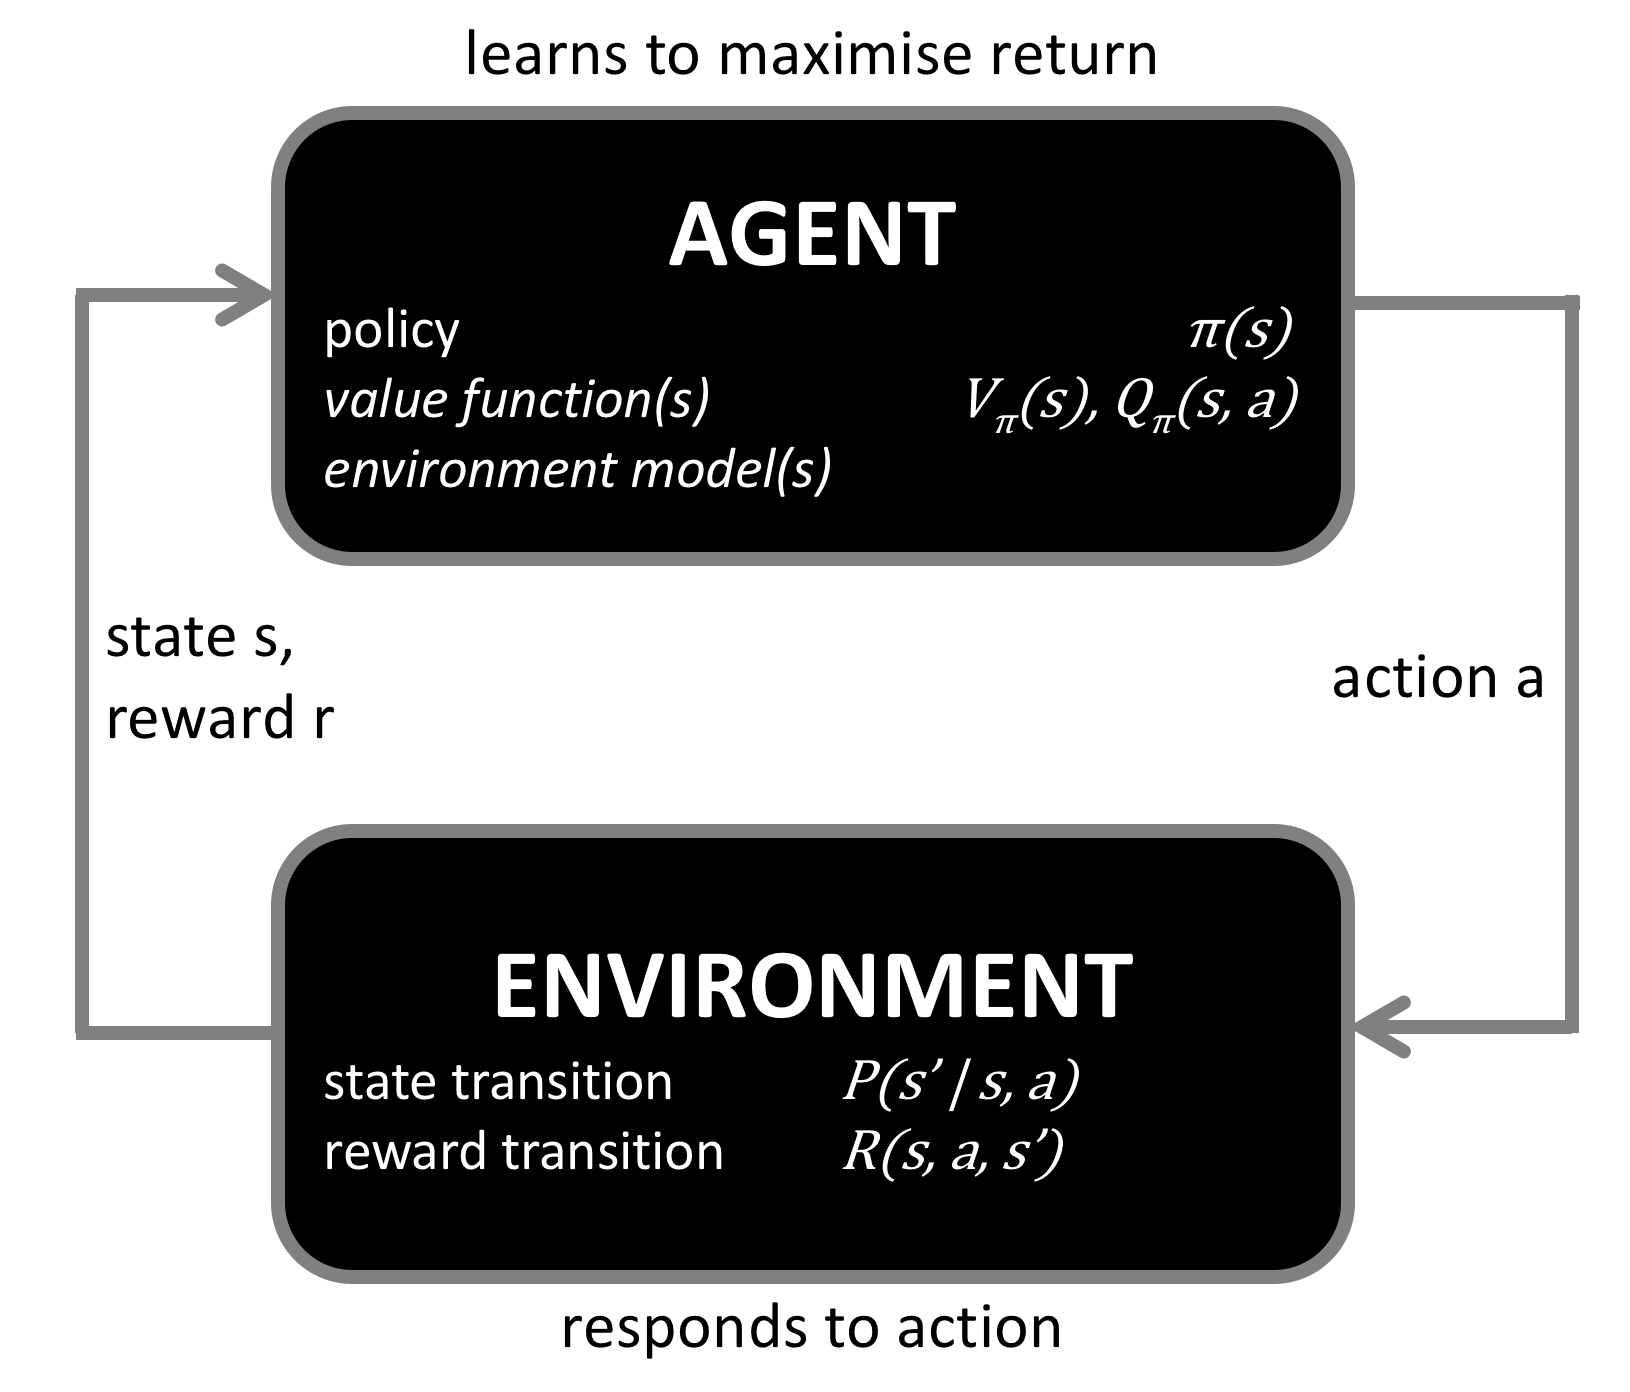
\includegraphics[width=\textwidth,height=0.5\textheight]{./tex2pdf.-4c1708fb449e9e84/a6864eb409708feab0fc8622776c8f177fe15c63.png}
\caption{The Markov Decision Process showing the agent and environment
internals}
\end{figure}

\newpage

\hypertarget{return}{%
\subsection{Return}\label{return}}

Goal of our agent is to maximize total reward - not just the next step
but. Return (\(G_t\)) is the total discounted future reward

\[ G_t = r_{t+1} + \gamma r_{t+2} + \gamma^2 r_{t+3} + ... = \sum_{k=0}^{\infty} \gamma^k r_{t+k+1} \]

The discount factor is exponential (usually set around 1.0 - 0.9) -
rewards in the future become much less valuable than reward sooner.

\hypertarget{why-discount}{%
\subsubsection{Why discount}\label{why-discount}}

Future is uncertain = stochastic environment (or maybe even a stochastic
policy!).

Matches human thinking - we use hyperbolic discounting in our decision
making. Our discount rates are also variable (based on
environmentalstimulus).

Finance = time value of money. Money is more valuable today than in a
years time because I can invest that money today and earn one years
interest on it.

Makes the maths work = the discount rate allows the finite and infinite
horizion problems to be united in the same framework.

\begin{itemize}
\tightlist
\item
  return for infinite horizon problems finite
\item
  discount rate is \([0,1)\)
\item
  can make the sum of an infinite series finite
\item
  this is a geometric series
\end{itemize}

Can use discount = 1 for games with tree-like structures (without
cycles), or when time to solve is irrelevant (i.e.~a board game).

\newpage

\hypertarget{four-central-challenges}{%
\subsection{Four central challenges}\label{four-central-challenges}}

\hypertarget{exploration-vs-exploitation}{%
\subsubsection{Exploration vs
exploitation}\label{exploration-vs-exploitation}}

Do I go to the restaurant in Berlin I think is best -- or do I try
something new?

\begin{itemize}
\tightlist
\item
  exploration = finding information
\item
  exploitation = using information
\end{itemize}

Agent needs to balance between the two

\begin{itemize}
\tightlist
\item
  we don't want to waste time exploring poor quality states
\item
  we don't want to miss high quality states
\end{itemize}

How stationary are the environment state transition and reward
functions?\\
How stochastic is my policy?

Design of reward signal vs.~exploration required

Time step matters

\begin{itemize}
\tightlist
\item
  too small = rewards are delayed = credit assignment harder
\item
  too large = coarser control
\end{itemize}

\hypertarget{data-quality}{%
\subsubsection{Data quality}\label{data-quality}}

IID = independent sampling \& identical distribution

RL breaks both in multiple ways

\textbf{Independent sampling} - all the samples collected on a given
episode are correlated (along the state trajectory) - our agent will
likely be following a policy that is biased (towards good states)

\textbf{Identically distributed} - learning changes the data
distribution - exploration changes the data distribution - environment
can be non-stationary

Reinforcement learning will \textbf{always} break supervised learning
assumptions about data quality

\hypertarget{credit-assignment}{%
\subsubsection{Credit assignment}\label{credit-assignment}}

The reward we see now might not be because of the action we just took

Reward signal can be - \textbf{delayed} - benefit/penalty of action only
seen much later\\
- \textbf{sparse} - experience with reward = 0

Can design a more dense reward signal for a given environment - reward
shaping - changing the reward signal can change behaviour

\hypertarget{sample-efficiency}{%
\subsubsection{Sample efficiency}\label{sample-efficiency}}

How quickly a learner learns

How often we reuse data - do we only learn once or can we learn from it
again - can we learn off-policy

How much we squeeze out of data - i.e.~learn a value function, learn a
environment model

Requirement for sample efficiency depends on how expensive it is to
generate data - cheap data -\textgreater{} less requirement for data
efficiency - expensive / limited data -\textgreater{} squeeze more out
of data

\end{document}
